\section{Method}
\label{sec:method}

\method{} instantiates the data-research loop in
Equations~\ref{eq:researchoutput}--\ref{eq:contextupdate}
(Figure~\ref{fig:framework}). Its two core
designs organize the research context $C_t$: a \emph{traceable behavioral map}
preserves task requirements and failure mechanisms with links to source
trajectories; \emph{target-conditioned context refinement} uses target-linked
feedback to build decision-ready context for comparing intended training,
actual RL experience, and target-evaluation outcomes.
Guided by this context, specification-driven
construction and independent review produce the environment--task--verifier
set $D_t$. The training-and-evaluation service remains fixed.

The following describes the maintained framework and labels a standalone
analysis refinement. Section~\ref{sec:experiments} distinguishes these from the earlier protocols
underlying the reported training curves.

\begin{figure}[t]
\centering
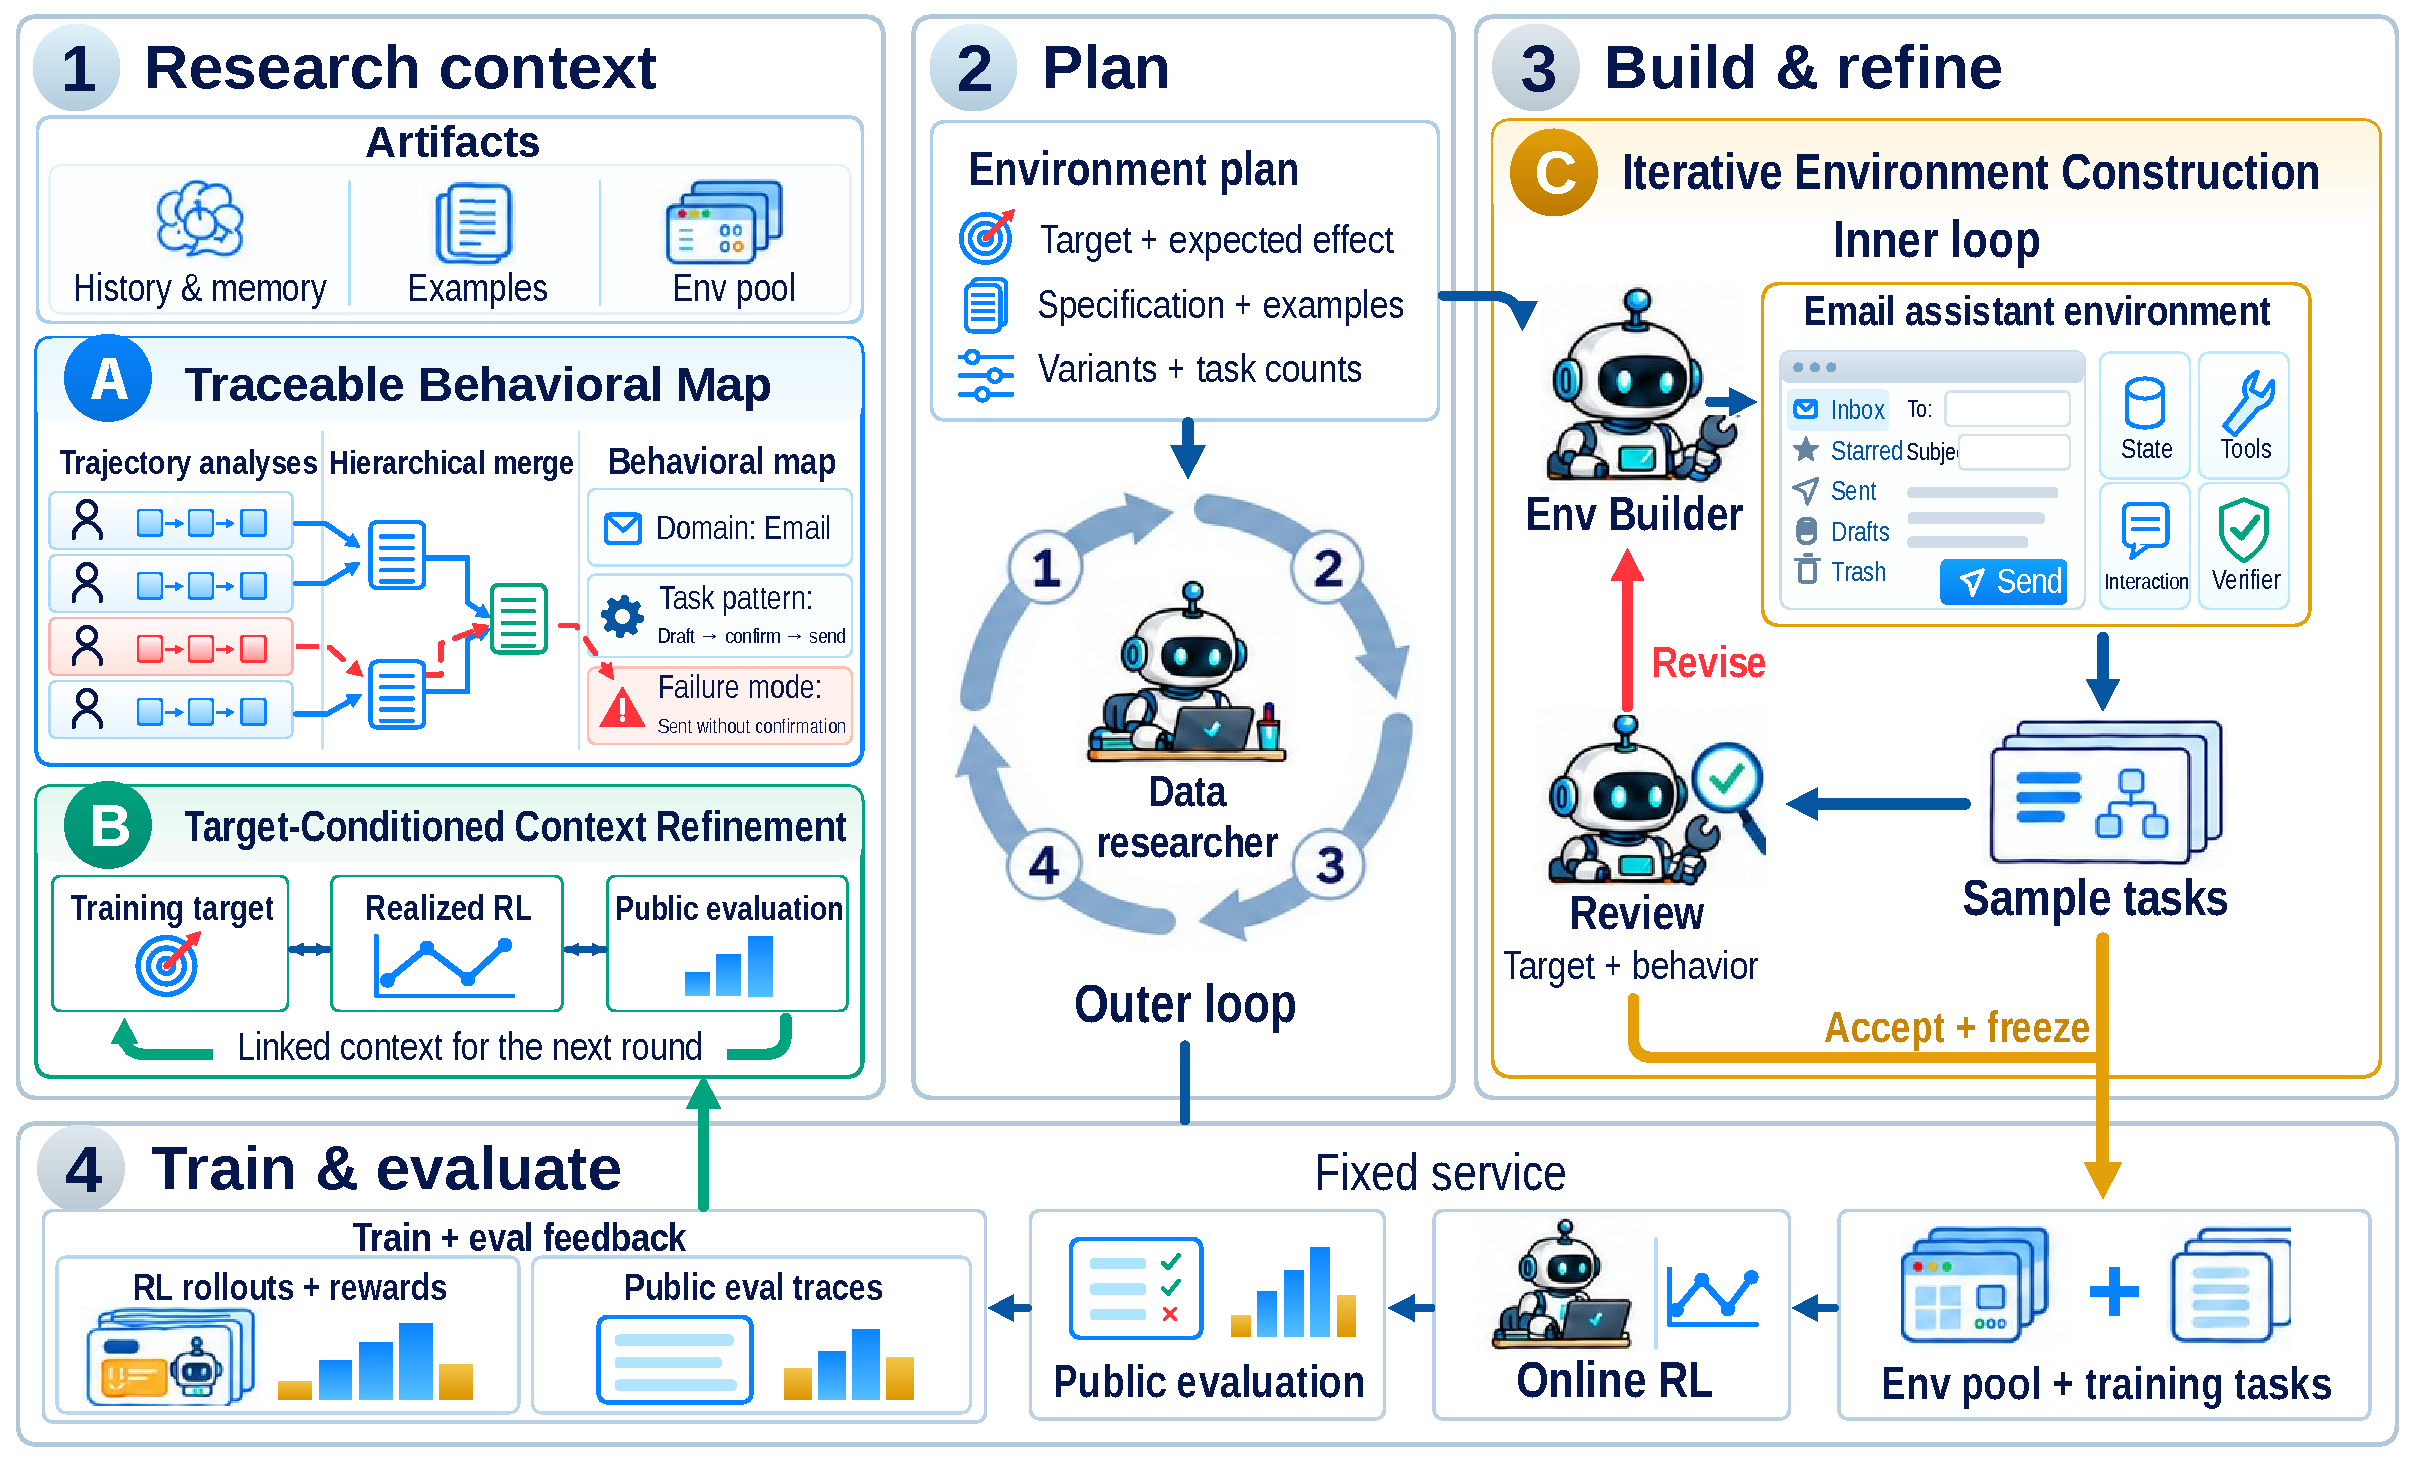
\includegraphics[width=\linewidth]{figures/framework.pdf}
\caption{\method{}'s research loop. A highlighted pattern traces back through the merge tree; linked target, training, and public-eval evidence guide the data researcher. Sampled tasks are independently reviewed and frozen before RL. Curves are schematic; B shows one historical example.}
\label{fig:framework}
\end{figure}


\subsection{Traceable Behavioral Map}
\label{sec:diagnosis}

The map separates a persistent evidence layer from its compact reading view.
Let $T_{t,i}$ contain the complete public-eval episodes for task $i$, including
instructions, tool definitions, and observed interactions. Extraction and
source review produce an immutable mechanism ledger:
\begin{equation}
\mathcal L_t=\bigcup_i \operatorname{ExtractReview}(T_{t,i}).
\label{eq:mechanismledger}
\end{equation}
Each record links an environment mechanism, task requirement, or observed
failure/recovery to its source and applicable conditions.

Bounded hierarchical merging builds a draft by factoring shared premises
while retaining distinct actors, scopes, dependencies, and recovery branches:
\begin{equation}
R_t^{(0)}=\operatorname{FactorMerge}(\mathcal L_t).
\label{eq:factoredmap}
\end{equation}
The draft is checked against the retained evidence, not only earlier
summaries. $\operatorname{Repair}$ locally corrects conflicting claims;
$\operatorname{Residual}$ extracts and consolidates only relations still
missing from the corrected report:
\begin{equation}
\begin{aligned}
\bar R_t &= \operatorname{Repair}(R_t^{(0)},\mathcal L_t),\\
R_t &= \bar R_t \oplus \operatorname{Residual}(\mathcal L_t,\bar R_t).
\end{aligned}
\label{eq:residualmap}
\end{equation}
Here $\oplus$ appends the missing distinctions without rewriting preserved
content; an already-covered record must instead be matched to an existing
passage. These are model-based checks, not a semantic-completeness guarantee.

The report retains the four fields \emph{domain, environment, task behavior,
failure behavior}. It enters the research context $C_t$ with links back to
original trajectories. This coverage-checked variant
is evaluated offline in Section~\ref{sec:analysiscoverage}, separately from
the earlier analysis used in the historical training runs.

\subsection{Target-Conditioned Context Refinement}
\label{sec:planning}

Access to evidence does not ensure its use in research decisions. We target
this \emph{information-utilization gap} with \emph{decision-ready context}:
evidence organized for joint interpretation around a shared behavioral target.
Our \emph{target-linked feedback} provides the context-level intervention,
explicitly connecting what was intended, what was trained, and how target
behavior changed.

For each intervention, the researcher declares a target requirement and
expected effect, anchored to public-eval tasks. Versioned triples in $D_t$
and their task IDs link this target to actual RL groups and rollouts,
forming a target-conditioned evidence view:
\begin{equation}
\underbrace{\text{Training target}}_{\text{requirement, expected effect}}
\longleftrightarrow
\underbrace{\text{Actual training}}_{\text{versioned triples, RL rollouts}}
\longleftrightarrow
\underbrace{\text{Target evaluation}}_{\text{linked public tasks}}.
\label{eq:lineage}
\end{equation}

The view distinguishes planned, accepted, and actually trained data, pairing
training-time reward statistics and within-task reward contrast with linked
public-eval outcomes and trajectories. The researcher compares these observations
with the expected effect, recording agreements, mismatches, and unresolved
questions in $C_{t+1}$. This assessment guides revisions to mechanisms,
challenge, or sampling, and decisions to retain or pause environments. The
design guides evidence use rather than adding otherwise inaccessible feedback;
the links do not establish causal effects of individual edits.

\subsection{Iterative Environment Construction}
\label{sec:environment}

We construct training environments through an iterative cycle of planning,
implementation, and review, revising either the implementation or the plan as
needed. The researcher selects training targets and task allocations, then
provides specifications with success, failure, and recovery
cases. Persistent Env Builders receive these specifications rather than raw
public-eval or RL corpora.

\label{sec:checks}
Each builder implements candidate $(e,x,v)$ triples, with task requests and
verifiers sharing the same goal data. Execution checks and independent review
examine the specification, full program, and all tasks in the batch. They
assess whether the intended decisions and variations are implemented and
whether information access, tool effects, and verifier rewards are consistent.
Implementation findings return to
the same builder for revision and renewed review, retaining prior findings;
specification ambiguities return to the researcher to revise the plan.

Accepted triples are frozen and retained while the researcher replans any
remaining allocations, subject to construction budgets. The accepted set
$D_t$ enters training once its admission requirement is met. This local
construction cycle precedes the outer training and feedback loop; review
remains fallible, not a proof of program correctness.
